\chapter{Casi d'Uso}

\todo{rivedere la numerazione dei casi d'uso}

\section{Inizializzazione del sistema}
\begin{figure}[h]
  \centering
  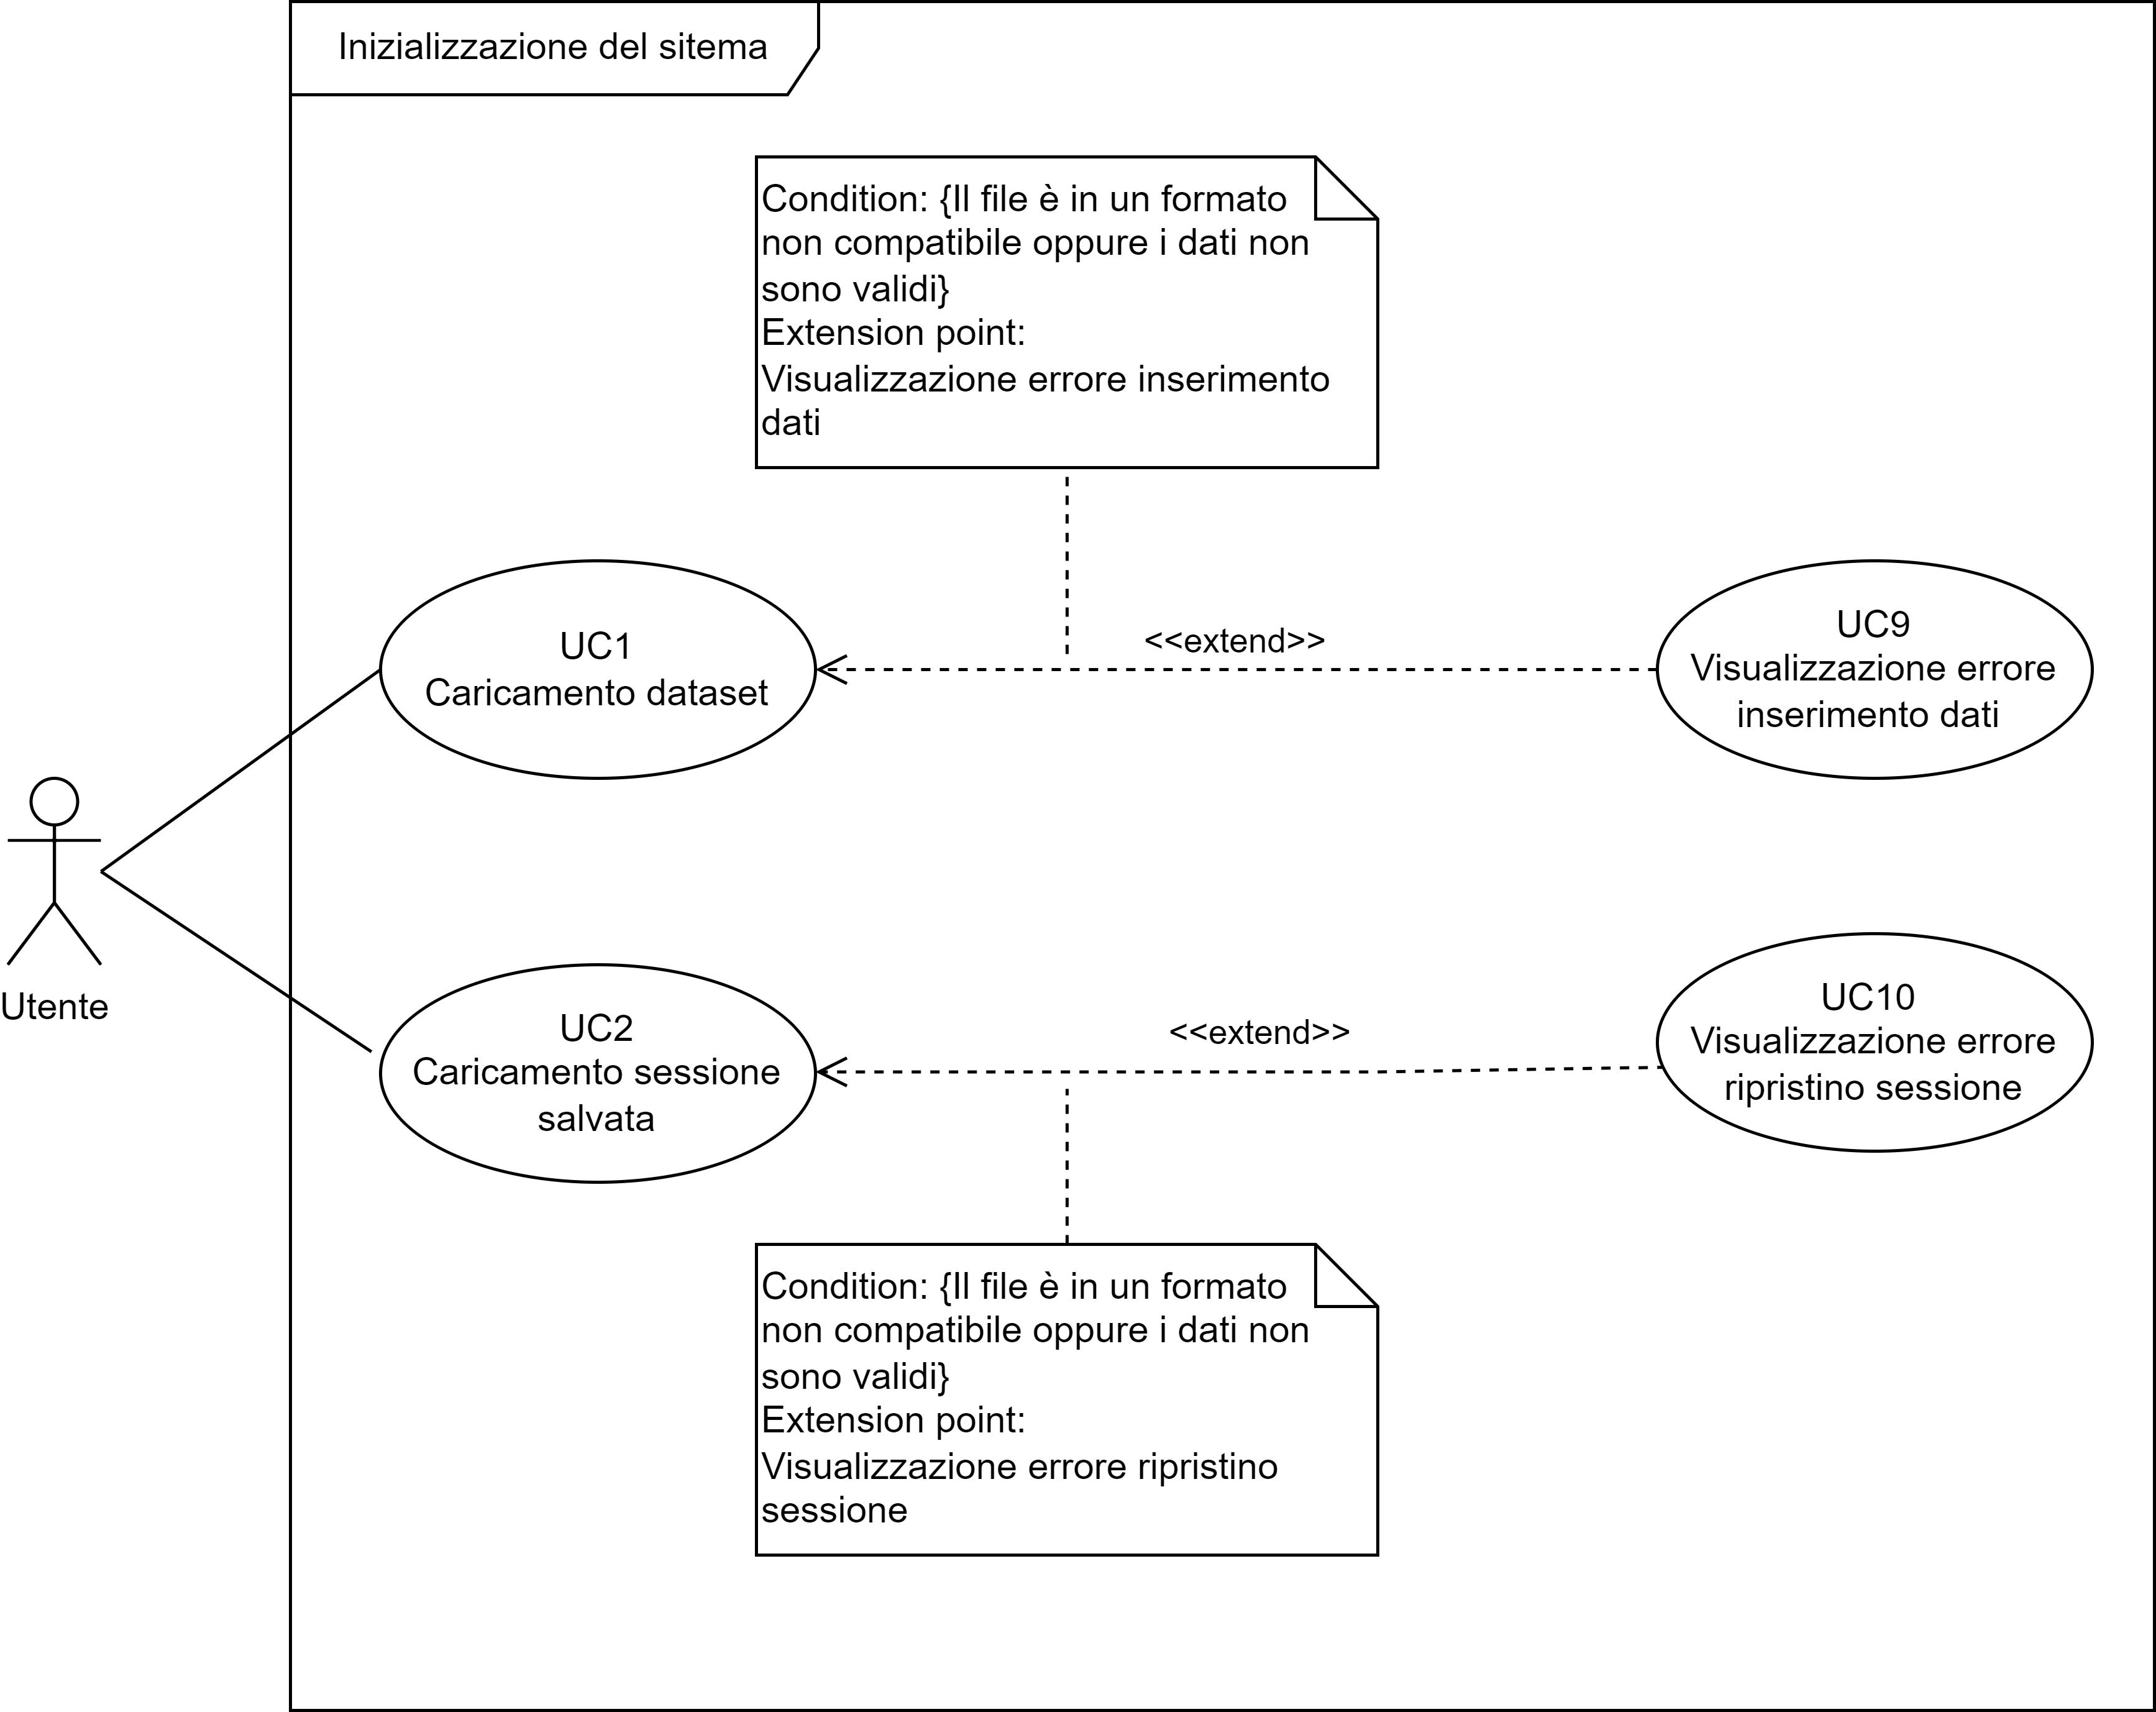
\includegraphics[width=0.6\textwidth]{Iniz_sistema}
  \caption{Inizializzazione del sistema}
\end{figure}
\subsection{UC1 - Caricamento dataset}
\begin{itemize}
  \item \textbf{Descrizione:} L'utente vuole analizzare un nuovo dataset non presente nel sistema;
  \item \textbf{Attore primario:} Utente;
  \item \textbf{Precondizioni:} Il sistema è raggiungibile e funzionante. L’utente ha a disposizione un dataset in formato CSV;
  \item \textbf{Postcondizioni:} I dati presenti nel file vengono caricati nel sistema. Viene visualizzato un messaggio che indica il corretto caricamento dei dati;
  \item \textbf{Scenario principale:}
  \begin{enumerate}
    \item L'utente accede al sistema;
    \item L'utente sceglie un file in formato CSV presente in locale e lo carica nel sistema;
    \item L'utente è pronto ad analizzare i dati.
  \end{enumerate}
  \item \textbf{Estensioni:}
    Nel caso in cui il file sia in un formato non valido o i dati non siano validi:
    \begin{enumerate}
      \item Il caricamento non va a buon fine;
      \item Viene visualizzato un errore esplicativo [UC3].
    \end{enumerate}
\end{itemize}
\subsection{UC2 - Caricamento sessione salvata}
\begin{itemize}
  \item \textbf{Descrizione:} L'utente vuole riprendere ad analizzare da dove si era interrotto
  o ha la necessità di visualizzare una sessione precedente;
  \item \textbf{Attore Primario:} Utente;
  \item \textbf{Precondizioni:} L'utente che avvia l'applicativo ha salvato almeno una sessione di lavoro precedente;
  \item \textbf{Postcondizioni:} I dati di una sessione precedentemente salvata vengono ricaricati nel sistema. Viene visualizzato un messaggio che indica il corretto caricamento dei dati;
  \item \textbf{Scenario Principale:}
  \begin{enumerate}
    \item L'utente accede al sistema;
    \item L'utente sceglie la sessione da caricare selezionando il file JSON desiderato tra quelli disponibili,
    cioè tra le sessioni salvate in precedenza;
    \item L'utente riprende da dove aveva salvato.
  \end{enumerate}
  \item \textbf{Estensioni:}
  Nel caso in cui il file JSON selezionato non è leggibile per qualche possibile errore di salvataggio:
    \begin{enumerate}
      \item Fallisce il caricamento della sessione precedente;
      \item Viene visualizzato un errore esplicativo [UC4].
    \end{enumerate}
  \end{enumerate}
\end{itemize}
\subsection{UC3 - Visualizzazione errore inserimento dati}
\begin{itemize}
  \item \textbf{Attore Primario:} Utente;
  \item \textbf{Precondizioni:} L'utente carica nel sistema un file CSV mal formattato o contenente dei dati non validi;
  \item \textbf{Postcondizioni:} L'utente visualizza un messaggio di errore e non viene caricato nessun file.
  \item \textbf{Scenario Principale:}
  \begin{enumerate}
    \item L'utente visualizza un messaggio di errore esplicativo;
    \item L'utente clicca \texttt{Capito} per tornare alla schermata iniziale.
  \end{enumerate}
\end{itemize}
\subsection{UC4 - Visualizzazione errore ripristino sessione}
\begin{itemize}
  \item \textbf{Attore Primario:} Utente;
  \item \textbf{Precondizioni:} L'utente ricarica una sessione che presenta un file JSON mal formattato o contenente dei valori per i parametri di configurazione non validi o non corretti;
  \item \textbf{Postcondizioni:} L'utente visualizza un messaggio di errore e la sessione non viene ricaricata.
  \item \textbf{Scenario Principale:}
  \begin{enumerate}
    \item L'utente visualizza un messaggio di errore esplicativo;
    \item L'utente clicca \texttt{Capito} per tornare alla schermata iniziale.
  \end{enumerate}

\section{UC3}

\section{UC4}

\section{UC5 - Accesso al Manuale Utente}
\begin{figure}[h]
  \centering
  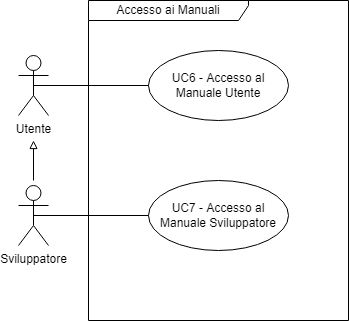
\includegraphics[width=0.6\textwidth]{UC_manuali}
  \caption{UC3 UC4 - Accesso ai manuali utente e sviluppatore}
\end{figure}

\begin{itemize}
  \item \textbf{Descrizione}: l'utente che ha un dubbio o vuole più informazioni sull'utilizzo dell'applicazione, deve avere accesso rapido al manuale utente;
  \item \textbf{Attore primario}: utente;
  \item \textbf{Precondizioni}: nessuna, l'opzione di accesso ai manuali deve essere sempre disponibile all'utente;
  \item \textbf{Postcondizioni}: viene visualizzato il manuale utente;
  \item \textbf{Scenario principale}: 
  \begin{enumerate}
    \item L'utente seleziona il "manuale utente";
    \item Viene visualizzato il manuale utente.
  \end{enumerate}
\end{itemize}

\section{UC5 + 1 - Accesso al Manuale Sviluppatore}

\begin{itemize}
  \item \textbf{Descrizione}: essendo Login Warrior un progetto open source, un qualsiasi utente deve avere accesso ad un manuale sviluppatore (sia per manutenere, sia per estendere il software);
  \item \textbf{Attore primario}: utente;
  \item \textbf{Precondizioni}: nessuna, l'opzione di accesso ai manuali deve essere sempre disponibile all'utente;
  \item \textbf{Postcondizioni}: viene visualizzato il manuale sviluppatore;
  \item \textbf{Scenario principale}: 
  \begin{enumerate}
    \item L'utente seleziona il "manuale sviluppatore";
    \item Viene visualizzato il manuale sviluppatore.
  \end{enumerate}
\end{itemize}

\section{UC6}

\section{UC7}
